%----------------------------------------------------------------------------------------
%	PACKAGES AND DOCUMENT CONFIGURATIONS
%----------------------------------------------------------------------------------------
\documentclass[article, a4paper, 11pt, oneside]{memoir}

% Margins
\usepackage[top=3cm,left=2cm,right=2cm,bottom=3cm]{geometry}

% Encondings
\usepackage[utf8]{inputenc}

% Language
\usepackage[portuguese]{babel}

% Graphics and images
\usepackage{graphicx}
	\graphicspath{{../images/}}

% Tables
\usepackage{tabularx}

% Paragraph Spacing
\usepackage{parskip}
\usepackage{indentfirst}
\setlength{\parskip}{0.4cm}

% Hyperreferences
\usepackage{hyperref}

% Repeated commands
\usepackage{expl3}
\ExplSyntaxOn
\cs_new_eq:NN \Repeat \prg_replicate:nn
\ExplSyntaxOff

% Header and Footer Things
\usepackage{wallpaper}
\usepackage{fancyhdr}

% Following code to edit the pagestyle
\pagestyle{fancy}
\fancyhf{}
\rhead{RCOM}
\rfoot{Página \thepage}

% Commands
\usepackage{xargs}

%% Linked Email
\newcommand{\email}[1]{
{\texttt{\href{mailto:#1}{#1}} }
}

% Code
\usepackage{listings}
\lstset{language=C}
\usepackage{color}
\definecolor{dkgreen}{rgb}{0,0.6,0}
\definecolor{gray}{rgb}{0.5,0.5,0.5}
\definecolor{mauve}{rgb}{0.58,0,0.82}

\lstset{frame=tb,
  language=C,
  aboveskip=3mm,
  belowskip=3mm,
  showstringspaces=false,
  columns=flexible,
  basicstyle={\small\ttfamily},
  numbers=none,
  numberstyle=\tiny\color{gray},
  keywordstyle=\color{blue},
  commentstyle=\color{dkgreen},
  stringstyle=\color{mauve},
  breaklines=true,
  breakatwhitespace=true,
  tabsize=3
}

%----------------------------------------------------------------------------------------
%	DOCUMENT INFORMATION
%----------------------------------------------------------------------------------------
% Title
\title{\Huge \texttt{Relatório do 2º Trabalho Laboratorial} }
% Authors
\author{
\LARGE \textbf{Grupo 5}\\\\
\begin{tabular}{l r}
	\email{up201806551@fe.up.pt} & Beatriz Costa Silva Mendes			\\
	\email{up201806528@fe.up.pt} & Clara Alves Martins		            \\
\end{tabular}
}


%\institute{Faculdade de Engenharia da Universidade do Porto - RCOM}

% Date for the report
\date{\today}

% Table of Contents
\addto\captionsportuguese{\renewcommand*\contentsname{Índice}}

%----------------------------------------------------------------------------------------
%	DOCUMENT
%----------------------------------------------------------------------------------------
\begin{document}
%----------------------------------------------------------------------------------------
%	Front Page
%----------------------------------------------------------------------------------------
% Title Author and Date
\maketitle

% More information for front page
\begin{center}
\textbf{Redes de Computadores - 2020/21 - MIEIC}
\Repeat{2}{\linebreak}
\begin{tabular}{l r}
	\textbf{Professor das Aulas Laboratoriais}: & Manuel Alberto Pereira Ricardo
\end{tabular}
\Repeat{4}{\linebreak}
% FEUP Logo

\includegraphics[scale=0.4]{img/FEUPlogo.png}

\end{center}

\newpage
% Header Image
\CenterWallPaper{0.1}{img/FEUPlogo.png}
\addtolength{\wpXoffset}{-7.5cm}
\addtolength{\wpYoffset}{13.8cm}

%----------------------------------------------------------------------------------------
%	TABLE OF CONTENTS
%----------------------------------------------------------------------------------------
\tableofcontents*

\section*{Sumário}

Este relatório foi elaborado no âmbito da unidade curricular de Redes de Computadores. O
trabalho consiste na configuração e estudo de uma rede de computadores. Este documento 
subdivide-se em diversas secções, destacando-se duas delas:
\begin{itemize}
  \item A aplicação de \textit{download}, onde é descrita a sua arquitetura e apresentados
os resultados da sua execução;
  \item A configuração da rede, onde são respondidas várias questões relativamente às
experiências realizadas e são analisados os resultados obtidos durante estas.
\end{itemize}
Assim sendo, o trabalho foi concluido com sucesso, visto que todos os objetivos foram 
cumpridos e foi finalizada uma aplicação capaz de transferir um ficheiro proveniente
de um servidor FTP.

\newpage

%----------------------------------------------------------------------------------------
%	CHAPTER 1 - Introdução
%----------------------------------------------------------------------------------------
\chapter[Introdução][Introdução]{Introdução} \label{\thechapter}

O segundo projeto de Redes de Computadores tem duas grandes finalidades: o \textbf{desenvolvimento 
de uma aplicação de \textit{download}} e a \textbf{configuração e estudo de uma rede de 
computadores}.

A \textbf{aplicação de \textit{download}} foi desenvolvida de acordo com o protocolo FTP (RFC 793) e 
com a ajuda de ligações TCP (\textit{Transmission Control Protocol}, RFC 793) a partir de 
\textit{sockets} de \textit{Berkeley}. Já relativamente à \textbf{configuração e estudo de uma 
rede de computadores}, o objetivo desta é permitir a execução de uma aplicação a partir de duas VLAN's 
dentro de um  \textit{switch}.

O relatório divide-se em:
\begin{enumerate}
  \item \textbf{Introdução}, onde são descritos os objetivos do trabalho prático;
  \item \textbf{Aplicação de Download}, onde é descrita a aplicação de \textit{download}, a sua 
arquitetura e os respetivos resultados obtidos;
  \item \textbf{Configuração da Rede e Análise}, onde é descrita a sua arquitetura, 
objetivos de cada experiência, comandos de configuração e análise dos resultados obtidos
durante a sua realização;
  \item \textbf{Conclusões}, onde é feita uma síntese da informação apresentada nas secções
anteriores e reflexão sobre os objetivos de aprendizagem alcançados;
  \item \textbf{Referências}, onde são colocados todos os documentos consultados para a realização 
deste trabalho;
  \item \textbf{Anexos}, onde se encontra o código fonte da aplicação desenvolvida e os resultados
obtidos durante as experiências.
\end{enumerate}

%----------------------------------------------------------------------------------------
%	CHAPTER 2 - Aplicação de Donwload
%----------------------------------------------------------------------------------------
\chapter[Aplicação de Download][Aplicação de Download]{Aplicação de Download} \label{\thechapter}

A primeira parte do segundo projeto de Redes de Computadores consiste no desenvolvimento de uma
aplicação de \textit{download} na linguagem de programação C. A aplicação desenvolvida aceita 
como argumento um link no seguinte formato: \verb|ftp://[<user>:<password>@]<host>/<url-path>|,
tendo sido estudado o RFC 959, que aborda o protocolo FTP, para a implementação desta aplicação.
O produto final consegue fazer \textit{download} de qualquer ficheiro de um servidor FTP. 

Posteriormente iremos descrever de forma sucinta a implementação da aplicação e as suas
funcionalidades, assim como os resultados obtidos e a sua análise.

\section{Arquitetura}

A aplicação desenvolvida pelo nosso grupo de trabalho está dividida em duas camadas: a de 
\textbf{processamento do URL} e a do \textbf{cliente FTP}. Estas duas camadas relacionam-se
apenas pelo facto da camada do cliente FTP utilizar a informação obtida no processamento do URL
para estabelecer conexões, enviar comandos e fazer o \textit{download} do ficheiro.

Primeiramente, é feito o processamento do URL. Para tal, são chamadas várias funções auxilares
que realizam o \textit{parse} da informação passada pelo argumento. As funções chamadas
para este efeito são:

\begin{itemize}
  \item \verb|parseArgs|: processa o argumento e coloca-o na estrutura de dados \verb|arguments|;
  \item \verb|parseFilename|: através do \textit{path} obtém-se o nome do ficheiro que se pretende
fazer o \textit{download};
  \item \verb|getIP|: obtém-se o IP a partir do \textit{hostname} passado como argumento.
\end{itemize}

Posteriormente, com o processamento do URL terminado, entra-se na camada do cliente FTP.
Inicialmente, é estabelecida a conexão, abrindo-se o \textit{socket}. Para abertura deste, é
necessário o IP obtido anteriormente e uma porta, que neste caso é a 21, a porta FTP,
tal como foi abordado nas aulas teóricas.

Depois da conexão, é necessário fazer-se a comunicação, passando-se vários argumentos através
do \textit{socket} pela seguinte ordem:

\begin{enumerate}
  \item \textbf{USER user}, envia-se o nome de utilizador para o servidor;
  \item \textbf{PASS pass}, envia-se a password para o servidor;
  \item \textbf{PASV}, entra-se em modo passivo, permitindo-se, assim, uma mútua comunicação
entre o servidor e o cliente FTP, sendo estabelecida numa nova conexão TCP. No
entando, agora o IP e a porta utilizados são as obtidas no modo passivo;
  \item \textbf{RETR filename}, é pedido ao servidor o envio do ficheiro para \textit{download}.
\end{enumerate}

Após o envio de todos estes comandos, é necessário fazer o \textit{download} do ficheiro. Para tal,
é chamada a função \verb|downloadFile|.

O código fonte da aplicação desenvolvida encontra-se no Anexo I. 

\section{Resultados de Donwload}

A aplicação desenvolvida pelo nosso grupo de trabalho foi testada em diversas condições: modo
anónimo, modo não anónimo, vários tipos de ficheiros, vários tamanhos de ficheiros, vários
servidores FTP, entre outros. Ao longo da execução é impresso no terminal informação sobre o
estado do programa para maior controlo por parte do utilizador.

Os resultados da execução do programa de \textit{download} podem ser visualizados em \ref{app}.

%----------------------------------------------------------------------------------------
%	CHAPTER 3 - Configuração da Rede e Análise
%----------------------------------------------------------------------------------------
\chapter[Configuração da Rede e Análise][Configuração da Rede e Análise]{Configuração da Rede e Análise} \label{\thechapter}

\section{\textbf{Experiência 1}: Configurar um IP de Rede}

O \textbf{ARP} (\textit{Address Resolution Protocol}) é um protocolo utilizado para descobrir 
dinamicamente a relação entre os endereços da camada 3 (protocolo) e da camada 2 
(\textit{hardware}). Normalmente esta relação estebelece-se entre um endereço IP e o seu
endereço de Ethernet, também designado por endereço MAC, podendo-se afirmar que
os pacotes ARP possuem toda esta informação.

O comando \textbf{\textit{ping}}, após a obtenção do endereço MAC através dos pacotes ARP, gera
pacotes do protocolo ICMP (\textit{Internet Control Message Protocol}) e espera por uma
resposta do \textit{target host}.

Antes de começar a experiência, foi necessário fazer a configuração das máquinas seguindo os passos
explicados em \ref{exp1-conf}.

Durante a execução desta experiência, foi necessário fazer o \textit{ping} do gnu 4 a partir do gnu 3.
Aquando deste, o gnu 3 envia um pacote ARP (\textit{request}) com o seu endereço IP (172.16.20.1),
o seu endereço MAC (00:21:5a:5a:78:c7), o endereço IP do destinatário (172.16.20.254)
e o endereço MAC do destinatário. Como o endereço MAC do destinatário lhe é desconhecido,
ele preenche este campo com 00:00:00:00:00:00. Posteriormente, obtém um pacote de resposta
(\textit{reply}) com os endereços de envio do gnu 4, IP (172.16.20.254) e MAC (00:22:64:a7:26:a2),
e os endereços de destino do gnu 3, IP (172.16.20.1) e MAC (00:21:5a:5a:78:c7).
Pode-se ver um exemplo destes pacotes em \ref{exp1-arp}.

Ao se dar \textit{ping} do gnu 4 a partir do gnu 3, os endereços IP e MAC obtidos serão
os correspondentes a cada um destes gnu's. Assim sendo, segue-se detalhadamente a informação
em relação aos endereços tanto do pacote de pedido como do pacote de resposta:

\textbf{Pacote de Pedido (ICMP \textit{request})}:

\begin{tabular}{||c c||} 
  \hline
    & Endereço \\ [0.5ex] 
  \hline\hline
  IP de Envio & 172.16.20.1  \\ 
  \hline
  MAC de Envio & 00:21:5a:5a:78:c7 \\
  \hline
  IP do destinatário & 172.16.20.254 \\
  \hline
  MAC do destinatário & 00:22:64:a7:26:a2 \\ [1ex] 
  \hline
\end{tabular}

\textbf{Pacote de Resposta (ICMP \textit{reply})}:

\begin{tabular}{||c c||} 
  \hline
    & Endereço \\ [0.5ex] 
  \hline\hline
  IP de Envio & 172.16.20.254  \\ 
  \hline
  MAC de Envio & 00:22:64:a7:26:a2 \\
  \hline
  IP do destinatário & 172.16.20.1 \\
  \hline
  MAC do destinatário & 00:21:5a:5a:78:c7 \\ [1ex] 
  \hline
\end{tabular}

Tal como se pode verificar, os pacotes ARP e os pacotes ICMP (\ref{exp1-icmp}) possuem informações
diferentes. Deste modo, para se poder distinguir entre eles, utiliza-se a \textbf{desmultiplexagem}.
O \textit{Ethernet header} presente nas tramas permite-nos distinguir tramas ARP de tramas IP.
Além disso, o IP \textit{header} presente nestas últimas permite-nos fazer a
distinção entre tramas ICMP e outras tramas IP. Esta distinção também pode ser feita através da leitura
dos resultados obtidos no \textit{wireshark}.
Analisando os resultados obtidos, é possível verificar-se que, quando o pacote tiver no
parâmetro "\textit{type}" o valor 0x0800 (\ref{exp1-ip-800}), significa que o tipo da trama é IP.
Posteriormente, é possível analisar o IP \textit{header}: se este tiver o valor 1 (\ref{exp1-icmp-1}),
significa que o tipo de protocolo é ICMP. Por outro lado, se o pacote tiver no parâmetro
"\textit{type}" o valor 0x0806 (\ref{exp1-arp-806}), então a trama é do tipo ARP.

Para se visualizar o comprimento da trama recetora, é necessário consultar o pacote
ICMP \textit{reply} e verificar a \textit{frame length}. No caso na experiência realizada
pelo nosso grupo de trabalho, esta tem o valor de 98 \textit{bytes}
(784 \textit{bits}) (\ref{exp1-frame}).

A interface de \textit{loopback} é uma interface de rede virtual que permite ao computador enviar pacotes
a si próprio. Esta interface é usada para diagnóstico e identificação de problemas na ligação à rede.

\section{\textbf{Experiência 2}: Implementar duas LAN's virtuais no \textit{switch}}

Nesta experiência, o objetivo principal era criar duas LAN's virtuais (\verb|vlany0| e \verb|vlany1|)
no \textit{switch}, sendo que os gnu's 3 e 4 foram associados à \verb|vlany0| e o gnu 2 foi 
associado à LAN \verb|vlany1|.

Toda a configuração feita nesta experiência pode ser observada em \ref{exp2-conf}.

Existem dois domínios de broadcast, correspondentes a cada uma das vlans.
Ao efetuarmos um \textit{ping} em \textit{broadcast} (\textit{ping -b (...)}) a partir do gnu 3,
não obtemos nenhuma resposta, tal como se pode verificar nos registos (\ref{exp2}). Isto acontece
porque, por predefinição, o \textit{ping} em \textit{broadcast} não obtém nenhuma resposta.

\section{\textbf{Experiência 3}: Configurar um Router em Linux}

Na experiência 3, foi configurado o gnu 4 como um \textit{router}, estabelecendo-se, assim, 
uma ligação entre as duas VLANs criadas na experiência 2. A configuração necessária para a 
experiência pode ser observada em \ref{exp3-conf}.

\begin{center}
  GNUY2
  \begin{tabular}{||c c||} 
  \hline
  Destino & Gateway \\ [0.5ex] 
  \hline\hline
  172.16.Y0.0 & 172.16.Y1.253  \\ 
  \hline
  172.16.Y1.0 & 0.0.0.0 \\ [1ex] 
  \hline
 \end{tabular}
\end{center}


 \begin{center} 
  GNUY3
  \begin{tabular}{||c c||} 
  \hline
  Destino & Gateway \\ [0.5ex] 
  \hline\hline
  172.16.Y0.0 & 0.0.0.0 \\ 
  \hline
  172.16.Y1.0 & 172.16.Y1.254 \\ [1ex] 
  \hline
 \end{tabular}
\end{center}


 \begin{center}
  GNUY4
  \begin{tabular}{||c c||} 
  \hline
  Destino & Gateway \\ [0.5ex] 
  \hline\hline
  172.16.Y0.0 & 0.0.0.0  \\ 
  \hline
  172.16.Y1.0 & 0.0.0.0 \\ [1ex] 
  \hline
 \end{tabular}
\end{center}

Uma tabela de \textit{forwarding} mapeia endereços de destino para os links de saída destes.
Assim, contém os endereços IP, e respetiva máscara, de forma a permitir que o pacote,
chegado ao router, seja encaminhado para o router adjacente adequado.

Nos registos do gnu 3, podem ser observadas mensagens de ARP com a finalidade de descobrir o endereço
MAC para onde reencaminhar os pacotes. Neste caso, o endereço MAC recebido é, em todos os casos,
00:21:5a:5a:74:3e (o endereço MAC do gnu 4 na VLAN y0). O endereço MAC recebido não é, de facto,
o endereço MAC do destino, mas sim o endereço MAC do router que permite alcançar o destino.

No caso do primeiro \textit{ping} 172.16.y0.254, o endereço MAC recebido é o endereço MAC do destino.
No entanto, tanto no \textit{ping} 172.16.y1.253 e \textit{ping} 172.16.y1.1, o endereço MAC
recebido é o endereço MAC do gnu 4 na VLAN y0, que, apesar de não ser o destinatário,	estabelece uma
ligação entre ambas as VLANs, fornecendo assim um caminho para o reencaminhamento das mensagens
destinadas aos computadores gnu 4 e gnu 2, ambos na VLAN y1, inacessíveis ao gnu 3 na VLAN y0.
\ref{exp3-arp}

Ao efetuar o comando \textit{ping}, também podemos observar pacotes ICMP.
Ao observarmos os pacotes ICMP do gnu 3 iremos reparar que, embora o endereço MAC que lhes está
associado seja sempre o mesmo (o endereço MAC do gnu 4 na VLAN y0), já que todos os
pacotes são encaminhados para este computador, o endereço IP não é sempre igual,
visto este depender do destinatário do pacote.
Podemos observar dois tipos de pacotes ICMP, pacotes de \textit{request} e pacotes de \textit{reply}.
Desta forma, podemos concluir que foi estabelecida uma ligação entre o gnu 3 na VLAN y0 e todas
as outras interfaces da rede.

\section{\textbf{Experiência 4}: Configurar um Router Comercial e Implementar o NAT}

Nesta experiência, o objetivo principal era configurar um \textit{router} comercial, inicialmente
sem NAT. Posteriormente, configurou-se o \textit{router} com NAT, de modo a permitir o acesso
à rede internet a partir dos computadores.

Toda a configuração feita nesta experiência, tanto do \textit{router} como do NAT,
pode ser observada em \ref{exp4-conf}.

Após a configuração do \textit{router}, os pacotes acabam por seguir as rotas estabelecidas
anteriormente. Se uma destas não existir, os pacotes são redirecionados para o \textit{router}
(\textit{default route}), e este informa quem enviou o pacote de que existe o gnu 4, sendo o pacote
posteriormente enviado através do gnu 4.

O NAT (\textit{Network Address Translation}) é usado na preservação de endereços,
sendo usado de forma a reutilizar endereços em múltiplos locais.
Este protocolo permite que endereços de IP privados e não registados se conectem à internet
através da transformação desses endereços num único endereço público e registado,
antes desses pacotes serem encaminhados para a rede pública.

\section{\textbf{Experiência 5}: DNS}

Na experiência 5, o objetivo principal é configurar o serviço DNS. Esta configuração faz-se 
através da edição do ficheiro \verb|resolv.conf| em todos os os \textit{hosts} da rede criada 
e pode ser observada em \ref{exp5-conf}.
O ficheiro \verb|resolv.conf| consiste num ficheiro utilizado em vários sistemas operativos
que configura o DNS. A única edição necessária ao ficheiro é inserir \verb|nameserver 172.16.1.1|,
que se trata do endereço IP do servidor que deve ser acedido (netlab.fe.up.pt).

O DNS abstrai endereços IP, tornando a sua utilização mais simples. Desta forma, o utilizador
não tem de lidar com os endereços IP numéricos nem com alterações nos mesmos (\ref{exp5-dns}).

Para testar esta configuração, fez-se \textit{ping} usando \textit{www.google.com}. Nos registos
verificou-se que, inicialmente, se envia um \textit{request} (\ref{exp5-dns-query}) da
informação contida neste domínio e, posteriormente, se recebe um pacote \textit{reply}
(\ref{exp5-dns-response}) com informação, nomeadamente o endereço IP do domínio,
comprovando-se que a configuração foi feita corretamente.

\section{\textbf{Experiência 6}: Conexões TCP}

Nesta experiência, o objetivo principal é utilizar a aplicação \textit{download} descrita na 
primeira parte do relatório para realizar o \textit{download} de um ficheiro.

A configuração desta experiência é igual à experiência 5, tal como se pode observar em
\ref{exp6-conf}.

Tal como foi explicado anteriormente, na aplicação desenvolvida pelo nosso grupo de trabalho são
abertas duas conexões TCP.
A primeira (aberta na porta FTP \textit{default}, 21) permite o envio de comandos FTP
ao servidor e receber as respetivas respostas, estabelecendo o controlo da informação.
A segunda conexão (aberta na porta recebida como reposta ao comando \verb|pasv|)
é usada para receber os dados do ficheiro enviado pelo servidor. 

Estas conexões são divididas em 3 fases: a abertura da conexão, o envio/receção de informação 
e o fecho da conexão. 

Inicialmente, o cliente envia um comando SYN para iniciar a conexão com o número de sequência X.
Posteriormente, o servidor, ao receber este comando, envia de volta para o cliente um novo comando SYN,
mas, desta vez, com um número de sequência Y e uma confirmação positiva (ACK) com o valor X+1.
De seguida, o cliente, ao receber a confirmação por parte do servidor, envia um novo comando SYN,
desta vez com um número de sequência de valor X+1 e uma confirmação positiva com o valor de Y+1.

Após esta troca de mensagens, a ligação entre o cliente e o servidor está estabelecida e pode
inicializar-se a transferência de dados. No final da transferência, é necessário fechar a conexão.
Este fecho inicia-se com o envio do comando FIN por parte do cliente com o número de sequência A.
O servidor, ao receber este comando, envia uma confirmação positiva de valor A+1. De seguida,
envia também o comando FIN para o cliente com uma confirmação positiva igual à enviada anteriormente.
Ao receber este último comando, o cliente envia uma confirmação positiva de valor B+1.
Por fim, a memória alocada para o processo é libertada. 

O mecanismo ARQ (\textit{Automatic Repeat Request}) é importante no controlo de erros durante a
transmissão de dados. Para isso, utiliza mensagens de \textit{acknowledge}
(mensagem enviada pelo recetor indicando a correta receção dos dados) e erros de \textit{timeout}
(erro ocurrido quando o tempo para receção de um pacote ACK expirou). O pacote irá ser
retransmitido até se atingir um número máximo de retransmissões ou até ser recebido um ACK
antes de acontecer \textit{timeout}. Neste caso, o método utilizado é uma variação do
\textit{Go-Back-N}. Assim, nos registos, podemos notar os parâmetros:
\begin{itemize}
  \item \textit{Sequence Number} - identifica o primeiro \textit{byte} de dados
  \item \textit{Acknowledgment Number} - identifica o último \textit{byte} de dados sem erros
  \item \textit{Window} - tamanho da janela, utilizado para o \textit{flow control}
  \item \textit{Checksum} - utilizado para a verificação da existência de erros
\end{itemize}

O mecanismo de controlo de congestão TCP (\ref{exp6-tcp},\ref{exp6-info}) utilizado é o
\textit{Slow Start}. Começando por enviar apenas um pacote, irá aumentar o número de pacotes
enviados simultaneamente de forma exponencial. Desta forma, assim que um pacote seja perdido,
o mecanismo irá detetar um congestionamento, procedendo de forma a diminuir esse congestionamento e
retransmitindo o pacote perdido. No caso de \textit{timeout}, o congestionamento é considerado severo,
recomeçando a transmissão, primeiro, em \textit{Slow Start} até à \textit{threshold}, e, depois,
em modo de \textit{Congestion Avoidance} até atingir um novo congestionamento.
No caso da receção de 3 ACKs, o congestionamento não é considerado severo, pelo que irá
imediatamente entrar no método de \textit{Congestion Avoidance}.
O método de \textit{Congestion Avoidance} consiste em ir aumentando, incrementalmente,
os pacotes transmitidos, até acontecer um congestionamento, diminuindo, nesse momento, o
número de pacotes transmitidos simultaneamente para metade.

Desta forma, tal como podemos verificar nos registos e no gráfico (\ref{exp6-6}) o ritmo de transferência
vai aumentando até se atingir um máximo, no qual ocorre timeout. Em seguida, o ritmo diminui
drasticamente, voltando depois a aumentar lentamente até existir um novo pico, e assim
sucessivamente, até ao final da transferência.

O aparecimento de uma segunda conexão TCP leva a uma queda na taxa de transmissão, uma vez
que a taxa de transferência passará a ser distribuída igualmente entre as duas conexões. \ref{exp6-6}

%----------------------------------------------------------------------------------------
%	CHAPTER 4 - Conclusões
%----------------------------------------------------------------------------------------
\chapter[Conclusões][Conclusões]{Conclusões} \label{\thechapter}

Após a realização do trabalho prático 2 da unidade curricular Redes de Computadores,
podemos afirmar que os conhecimentos adquiridos ao longo das aulas teóricas encontram-se
agora consolidados, nomeadamente o protocolo FTP, as conexões TCP, a configuração de
endereços de IP, a implementação de VLAN's em \textit{switch} e a configuração de um
\textit{router} comercial, com e sem NAT, e a configuração de um serviço de DNS.

Assim sendo, consideramos que os objetivos para este trabalho prático foram atingidos com
sucesso, uma vez que implementamos uma aplicação \textit{download} funcional numa
rede de computadores configurada ao longo das aulas práticas, apesar de todos as dificuldades
que acabaram por surgir tendo em conta o contexto atual de pandemia, nomeadamente em relação
ao horário reduzido para utilização dos laboratórios e a dificuldade acrescida de
apenas frequentarmos o laboratório em metade das aulas, devido à restrição de apenas um dos
membros do grupo poder frequentar simultaneamente o laboratório.

%----------------------------------------------------------------------------------------
%	CHAPTER 5 - Referências
%----------------------------------------------------------------------------------------
\chapter[Referências][Referências]{Referências} \label{\thechapter}

\hyperlink{https://en.wikipedia.org/wiki/List_of_FTP_server_return_codes}{FTP Responde Codes}

\hyperlink{https://moodle.up.pt/pluginfile.php/36774/mod_resource/content/6/network.pdf}{The 
Network Layer, Powerpoint Aulas Teóricas}

\hyperlink{https://wiki.wireshark.org/AddressResolutionProtocol}{ARP, Wireshark Wiki}

\hyperlink{James F. Kurose, Keith W. Ross, Computer Networking - a Top-Down Approach, 6th Edition, Pearson}{Forwarding Table, Computer Networking - a Top-Down Approach, by James F. Kurose and Keith W. Ross}

\hyperlink{https://www.cisco.com/c/en/us/td/docs/wireless/mwr_2941_dc/software_config/guide/3_4/2941_34_Config_Guide/ge_ifcs.html}{Configuring the Interface Properties, CISCO}

\hyperlink{https://www.cisco.com/c/en/us/support/docs/ip/network-address-translation-nat/26704-nat-faq-00.html}{NAT, CISCO}

\hyperlink{https://man7.org/linux/man-pages/man5/resolv.conf.5.html}{resolv.conf, Linux Manual Page}

\hyperlink{https://www.dns.pt/pt/dominio/o-sistema-dns/}{DNS, DNS pt}

\newpage

%----------------------------------------------------------------------------------------
%	CHAPTER 6 - Anexos
%----------------------------------------------------------------------------------------
\chapter[Anexos][Anexos]{Anexos} \label{\thechapter}

\section{Anexo I - Código Fonte}

\subsection{constraints.h}

\lstinputlisting[language=C]{../src/constraints.h}

\subsection{download.h}

\lstinputlisting[language=C]{../src/download.c}   

\subsection{auxfunctions.h}

\lstinputlisting[language=C]{../src/auxfunctions.c}

\subsection{parsing.h}

\lstinputlisting[language=C]{../src/parsing.c}

\newpage

\section{Anexo II - Configurações}


Devido às dificuldades que surgiram perante a situação atual de contexto de pandemia, o nosso
grupo de trabalho teve dificuldades em obter registos para todas as experiências. Assim sendo,
os registos analisados na experiência 1 foram obtidos por nós (Sala 320, Bancada 2) e nas 
restantes experiências analisamos os registos obtidos pelo grupo T6G8 (Sala 320, Bancada 3).

\subsection{Experiência 1} \label{exp1-conf}

\textbf{Cabos}
\begin{lstlisting}[language=bash]
GNUY3E0 -> Switch Port 1
GNUY4E0 -> Switch Port 2
\end{lstlisting}

\textbf{gnuY3}
\begin{lstlisting}[language=bash]
  ifconfig eth0 up
  ifconfig eth0 172.16.Y0.1/24
\end{lstlisting}

\textbf{gnuY4}
\begin{lstlisting}[language=bash]
  ifconfig eth0 up
  ifconfig eth0 172.16.Y0.254/24
\end{lstlisting}

\subsection{Experiência 2} \label{exp2-conf}

\textbf{Cabos}
\begin{lstlisting}[language=bash]
GNUY3E0 -> Switch Port 1
GNUY4E0 -> Switch Port 2
GNUY2E0 -> Switch Port 3
\end{lstlisting}

\textbf{gnuY2}
\begin{lstlisting}[language=bash]
  ifconfig eth0 up
  ifconfig eth0 172.16.Y1.1/24
\end{lstlisting}

\textbf{gnuY3}
\begin{lstlisting}[language=bash]
  ifconfig eth0 up
  ifconfig eth0 172.16.Y0.1/24
\end{lstlisting}

\textbf{gnuY4}
\begin{lstlisting}[language=bash]
  ifconfig eth0 up
  ifconfig eth0 172.16.Y0.254/24
\end{lstlisting}

\textbf{Switch}
\begin{lstlisting}[language=bash]
  configure terminal
  vlan y0
  end

  configure terminal
  interface fastethernet 0/1
  switchport mode access
  switchport access vlan y0
  end
  configure terminal
  interface fastethernet 0/2
  switchport mode access
  switchport access vlan y0
  end

  configure terminal
  vlan y1 
  end 

  configure terminal
  interface fastethernet 0/3
  switchport mode access
  switchport access vlan y1
  end
\end{lstlisting}

\subsection{Experiência 3} \label{exp3-conf}

\textbf{Cabos}
\begin{lstlisting}[language=bash]
GNUY3E0 -> Switch Port 1
GNUY2E0 -> Switch Port 2
GNUY4E0 -> Switch Port 3
GNUY4E1 -> Switch Port 4
\end{lstlisting}

\textbf{gnuY2}
\begin{lstlisting}[language=bash]
  ifconfig eth0 up
  ifconfig eth0 172.16.Y1.1/24

  route add -net 172.16.Y0.0/24 gw 172.16.Y1.253
\end{lstlisting}

\textbf{gnuY3}
\begin{lstlisting}[language=bash]
  ifconfig eth0 up
  ifconfig eth0 172.16.Y0.1/24

  route add -net 172.16.Y1.0/24 gw 172.16.Y0.254
\end{lstlisting}

\textbf{gnuY4}
\begin{lstlisting}[language=bash]
  ifconfig eth0 up
  ifconfig eth0 172.16.Y0.254/24

  ifconfig eth1 up 
  ifconfig eth1 172.16.Y1.253/24

  echo 1 > /proc/sys/net/ipv4/ip_forward
  echo 0 > /proc/sys/net/ipv4/icmp_echo_ignore_broadcasts
\end{lstlisting}

\textbf{Switch}
\begin{lstlisting}[language=bash]
  configure terminal
  vlan y0
  end

  configure terminal
  interface fastethernet 0/1
  switchport mode access
  switchport access vlan y0
  end

  configure terminal
  interface fastethernet 0/2
  switchport mode access
  switchport access vlan y0
  end

  configure terminal
  vlan y1 
  end 

  configure terminal
  interface fastethernet 0/3
  switchport mode access
  switchport access vlan y1
  end

  configure terminal
  interface fastethernet 0/4
  switchport mode access
  switchport access vlan y1
  end
\end{lstlisting}

\subsection{Experiência 4} \label{exp4-conf}

\textbf{Cabos}
\begin{lstlisting}[language=bash]
GNUY3E0 -> Switch Port 1
GNUY2E0 -> Switch Port 2
GNUY4E0 -> Switch Port 3
GNUY4E1 -> Switch Port 4
ROUTERE0 -> Switch Port 5
ROUTERE1 -> Shelf Port 1
\end{lstlisting}

\textbf{gnuY2}
\begin{lstlisting}[language=bash]
  ifconfig eth0 up
  ifconfig eth0 172.16.Y1.1/24

  route add -net 172.16.Y0.0/24 gw 172.16.Y1.253
\end{lstlisting}

\textbf{gnuY3}
\begin{lstlisting}[language=bash]
  ifconfig eth0 up
  ifconfig eth0 172.16.Y0.1/24

  route add -net 172.16.Y1.0/24 gw 172.16.Y0.254
\end{lstlisting}

\textbf{gnuY4}
\begin{lstlisting}[language=bash]
  ifconfig eth0 up
  ifconfig eth0 172.16.Y0.254/24

  ifconfig eth1 up 
  ifconfig eth1 172.16.Y1.253/24

  echo 1 > /proc/sys/net/ipv4/ip_forward
  echo 0 > /proc/sys/net/ipv4/icmp_echo_ignore_broadcasts
\end{lstlisting}

\textbf{Switch}
\begin{lstlisting}[language=bash]
  configure terminal
  vlan y0
  end

  configure terminal
  interface fastethernet 0/1
  switchport mode access
  switchport access vlan y0
  end

  configure terminal
  interface fastethernet 0/2
  switchport mode access
  switchport access vlan y0
  end

  configure terminal
  vlan y1 
  end 

  configure terminal
  interface fastethernet 0/3
  switchport mode access
  switchport access vlan y1
  end

  configure terminal
  interface fastethernet 0/4
  switchport mode access
  switchport access vlan y1
  end

  configure terminal
  interface fastethernet 0/5
  switchport mode access
  switchport access vlan y1
  end
\end{lstlisting}

\textbf{Router}
\begin{lstlisting}
  conf t
  interface fastethernet 0/0
  ip address 172.16.y1.254 255.255.255.0
  no shutdown
  ip nat inside
  exit

  interface fastethernet 0/1
  ip address 172.16.1.y9 255.255.255.0
  no shutdown
  ip nat outside
  exit

  ip nat pool ovrld 172.16.1.y9 172.16.1.y9 prefix 24
  ip nat inside source list 1 pool ovrld overload

  access-list 1 permit 172.16.y0.0 0.0.0.7
  access-list 1 permit 172.16.y1.0 0.0.0.7

  ip route 0.0.0.0 0.0.0.0 172.16.1.254
  ip route 172.16.y0.0 255.255.255.0 172.16.y1.253
  end
\end{lstlisting}

\subsection{Experiência 5} \label{exp5-conf}

Repetir passos da experiência 4, mas adicionar os seguintes comandos aos gnu's 2, 3 e 4.
\begin{lstlisting}[language=bash]
  echo $'search netlab.fe.up.pt\nnameserver 172.16.2.1' > /etc/resolv.conf
\end{lstlisting}

\subsection{Experiência 6} \label{exp6-conf}

Repetir passos da experiência 5.

\newpage

\section{Anexo III - Imagens}

\begin{figure}[htbp]  \label{app}
  \centering        
  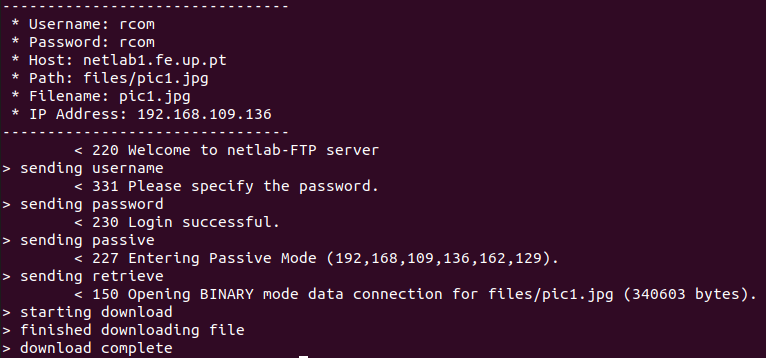
\includegraphics[scale=0.5]{img/app.png}
  \caption{Exemplo de execução da aplicação de \textit{download}}
\end{figure}

\begin{figure}[htbp]  \label{exp1-arp}
  \centering        
  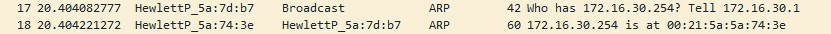
\includegraphics[scale=0.8]{img/exp1-arp.jpg}
  \caption{Exemplo de pacotes ARP}
\end{figure}

\begin{figure}[htbp]  \label{exp1-icmp}
  \centering        
  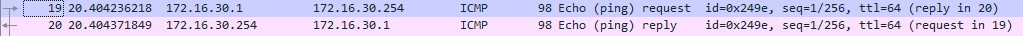
\includegraphics[scale=0.65]{img/exp1-icmp.jpg}
  \caption{Exemplo de pacotes ICMP}
\end{figure}

\begin{figure}[htbp]  \label{exp1-ip-800}
  \centering        
  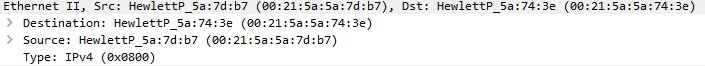
\includegraphics[scale=0.8]{img/exp1-ip-800.jpg}
  \caption{\textit{Type} de IP}
\end{figure}

\begin{figure}[htbp]  \label{exp1-icmp-1}
  \centering        
  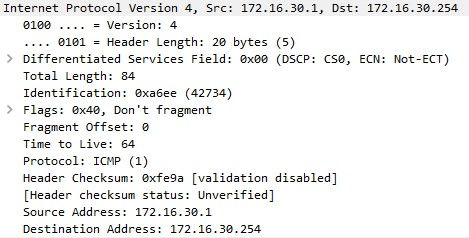
\includegraphics[scale=0.8]{img/exp1-icmp-1.jpg}
  \caption{\textit{Protocol} de ICMP}
\end{figure}

\begin{figure}[htbp]  \label{exp1-arp-806}
  \centering        
  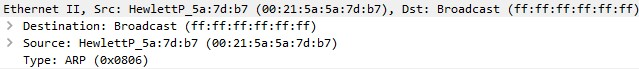
\includegraphics[scale=0.8]{img/exp1-arp-806.jpg}
  \caption{\textit{Type} de ARP}
\end{figure}

\begin{figure}[htbp]  \label{exp1-frame}
  \centering        
  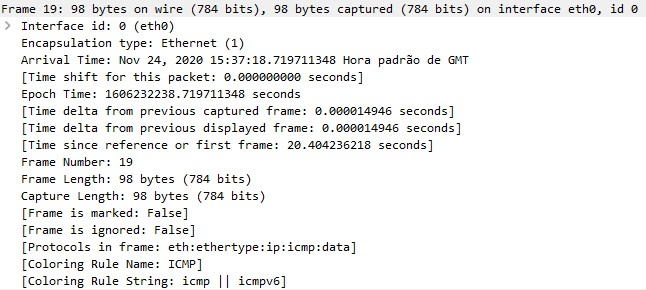
\includegraphics[scale=0.8]{img/exp1-frame.jpg}
  \caption{Exemplo da \textit{frame length} de um pacote ICMP}
\end{figure}

\begin{figure}[htbp]  \label{exp3-arp}
  \centering        
  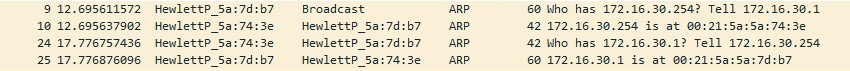
\includegraphics[scale=0.8]{img/exp3-arp.jpg}
  \caption{Pacotes ARP enviados entre o gnuY4 e o gnuY3}
\end{figure}

\begin{figure}[htbp]  \label{exp2}
  \centering        
  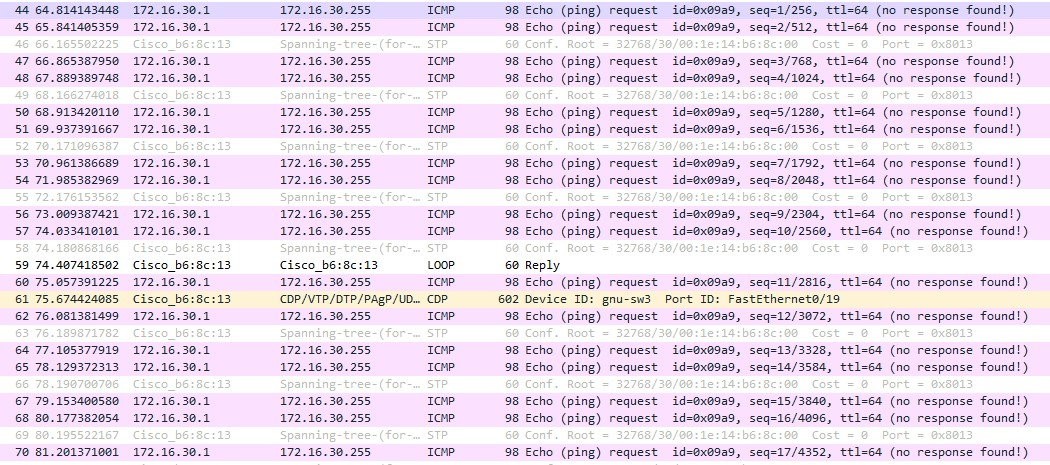
\includegraphics[scale=0.5]{img/exp2.jpg}
  \caption{Exemplo de Pacotes ICMP sem resposta}
\end{figure}

\begin{figure}[htbp]  \label{exp5-dns}
  \centering        
  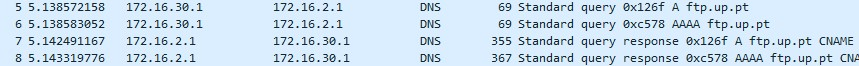
\includegraphics[scale=0.8]{img/exp5-dns.jpg}
  \caption{Pacotes DNS}
\end{figure}

\begin{figure}[htbp]  \label{exp5-dns-query}
  \centering        
  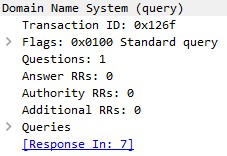
\includegraphics[scale=0.8]{img/exp5-dns-query.jpg}
  \caption{Parâmetros de um pacote DNS (1)}
\end{figure}

\begin{figure}[htbp]  \label{exp5-dns-response}
  \centering        
  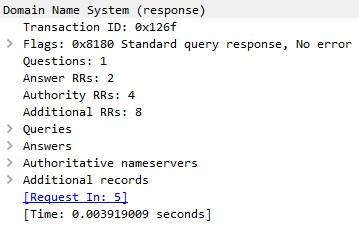
\includegraphics[scale=0.8]{img/exp5-dns-response.jpg}
  \caption{Parâmetros de um pacote DNS (2)}
\end{figure}

\begin{figure}[htbp]  \label{exp6-tcp}
  \centering        
  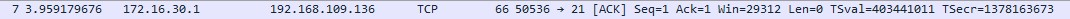
\includegraphics[scale=0.6]{img/exp6-tcp.jpg}
  \caption{Exemplo de um pacote TCP}
\end{figure}

\begin{figure}[htbp]  \label{exp6-info}
  \centering        
  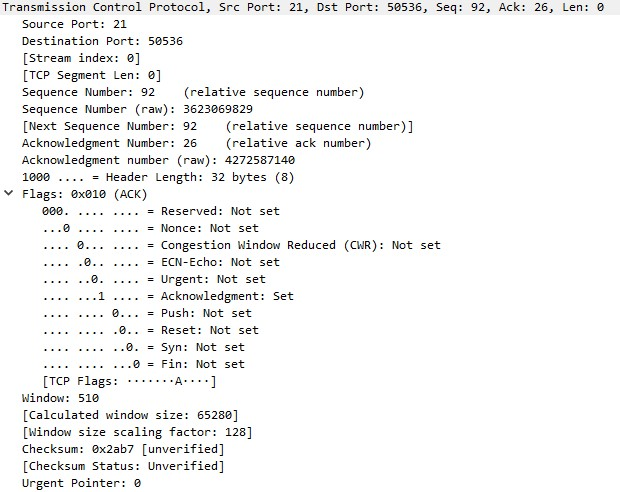
\includegraphics[scale=0.8]{img/exp6-info.jpg}
  \caption{Informação num pacote TCP}
\end{figure}

\begin{figure}[htbp]  \label{exp6-6}
  \centering        
  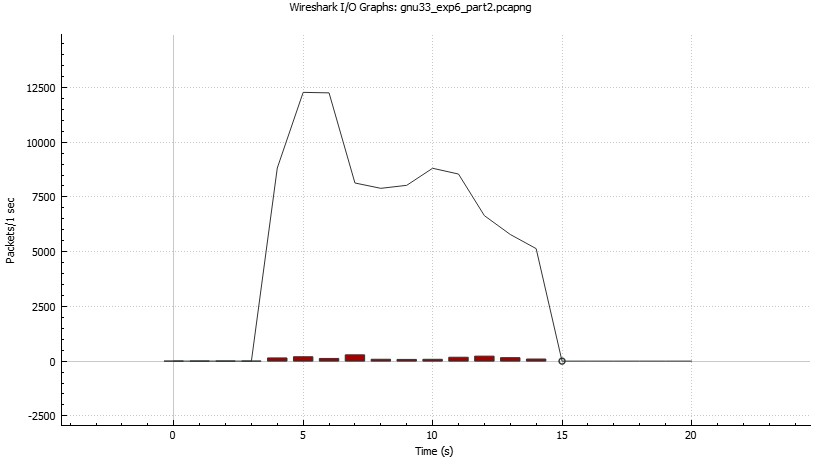
\includegraphics[scale=0.7]{img/exp6-6.jpg}
  \caption{Taxa de transferência FTP}
\end{figure}


\end{document}
